%=========================================================================
% (c) 2011, 2012 Josef Lusticky

\section{Hardware clock}\label{sec:analysis-hwclock}
On AVR Raven, Contiki uses the 8-bit Timer/Counter~2 module,
clocked from an asynchronous 32~768~Hz crystal oscillator, as the hardware clock by default.
The oscillator is independent of any other clock,
can only be used with Timer/Counter~2 and it
enables the use of Timer/Counter~2 as a Real Time Counter~\cite{avr-datasheet}.
The Timer/Counter~2 prescale value 8 is used in Contiki on the AVR Raven platform -
the oscillator frequency of 32~768~Hz is effectively divided by 8 and
the counter register is hence incremented with the frequency of
$f_{T2} = {\frac{f_{asy}}{prescaler}} = {\frac{32768}{8}} = 4096$~Hz.
Figure~\ref{fig:avr-clock} shows the Timer/Counter~2 module used by Contiki.
\begin{figure}
  \centering
  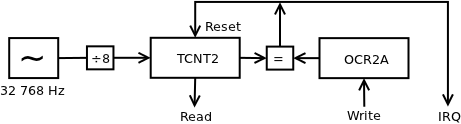
\includegraphics[width=9cm,keepaspectratio]{fig/avr-clock.png}
  \caption{Timer/Counter 2 hardware clock module on AVR Raven}
  \label{fig:avr-clock}
\end{figure}

The Timer/Counter~2 module is used in the Clear Timer on Compare Match (CTC) mode by Contiki.
In this mode, the counter register {\it{TCNT2}} is incrementing
and the compare register {\it{OCR2A}} defines the maximum value of the counter register.
A compare match between the counter register and the compare register
sets the Output Compare Flag {\it{OCF2A}} and resets the counter register to zero~\cite{avr-datasheet}.
This behaviour is illustrated in figure~\ref{fig:design-timing-diagram}
- the {\it{TOP}} value is equal to the value in the compare register and the {\it{BOTTOM}} value is equal to zero.

\begin{figure}
  \centering
  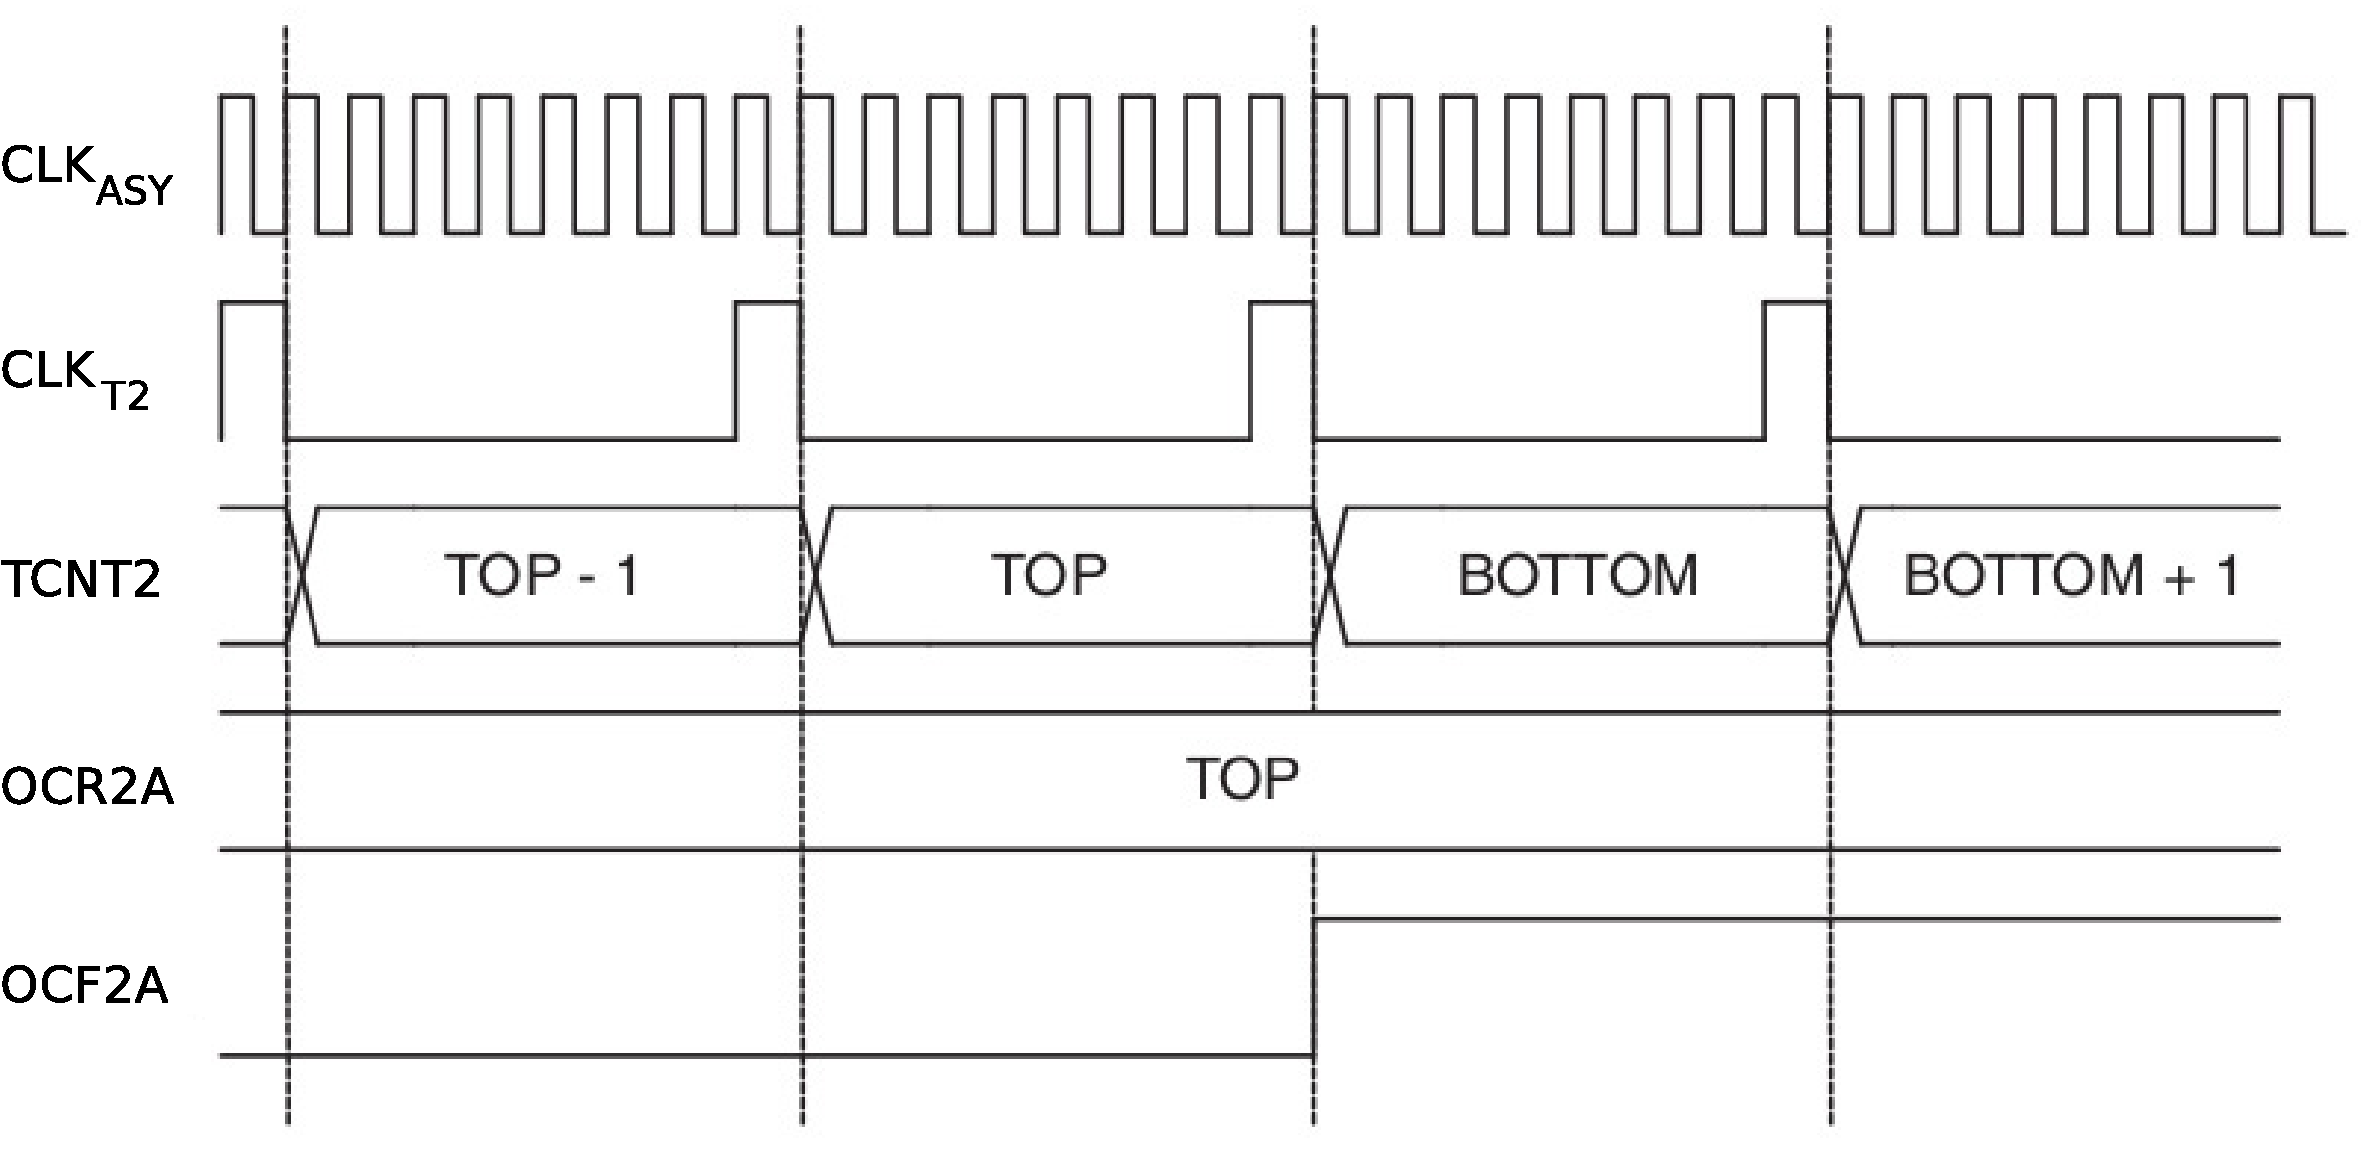
\includegraphics[width=12cm,keepaspectratio]{fig/timing-diagram.pdf}
  \caption{Timing diagram in CTC mode with prescaler 8 (source:~\cite{avr-datasheet})}
  \label{fig:design-timing-diagram}
\end{figure}

Additionally, when the compare match occurs,
an interrupt is raised and the interrupt service routine is executed.
The flag indicating occurred match {\it{OCF2A}} is
cleared automatically by hardware when executing
the interrupt service routine in this case~\cite{avr-datasheet}.

The interrupt service routine can be further used for updating the value in the {\it{OCR2A}} compare register.
However, changing {\it{OCR2A}} to a value closer to zero while the counter is running
must be done with care because the CTC mode does not have a double buffering feature.
If the new value written to {\it{OCR2A}} is lower than the current
value of {\it{TCNT2}}, the compare match will be missed~\cite{avr-datasheet}.
